\label{chap:system_design}

\section{Thiết kế kiến trúc hệ thống}
\label{sec:architecture_design}

Kiến trúc hệ thống xác định cấu trúc, các thành phần chính và mối quan hệ giữa chúng, nhằm đáp ứng các yêu cầu chức năng và phi chức năng. Hệ thống được thiết kế theo mô hình Client-Server với REST API module hóa, đảm bảo hiệu quả phát triển và dễ bảo trì.

\subsection{Kiến trúc tổng quan (Client-Server với REST API)}
\label{subsec:current_architecture_description}

Hệ thống tuân theo mô hình phân lớp client-server, Frontend là SPA (Single Page Application) giao tiếp với Backend qua REST API.

\begin{figure}[H]
    \centering
    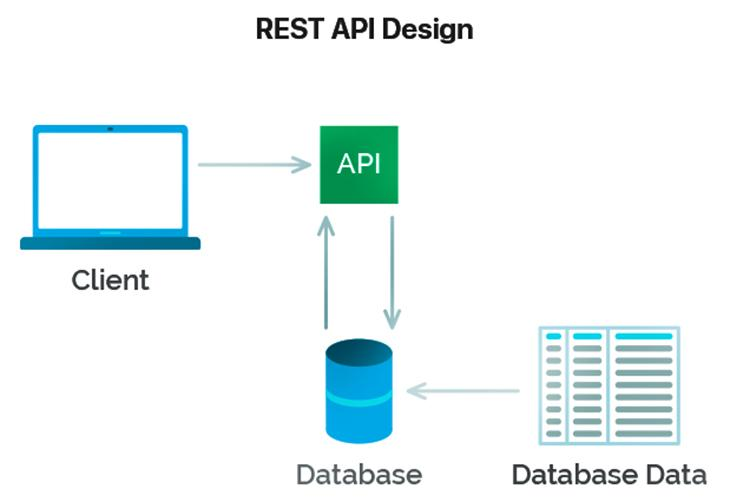
\includegraphics[width=0.75\textwidth]{Images/API.jpg}
    \vspace{1em}
    \caption{Mô hình kiến trúc Client-Server với REST API \cite{MicrosoftLearnClientServerImg}.}
    \label{fig:rest_api_architecture}
\end{figure}

\subsubsection{Frontend (Client)}
\label{subsubsec:frontend_component}
Frontend là lớp giao diện trực tiếp với người dùng, được xây dựng dưới dạng Single Page Application (SPA) để mang lại trải nghiệm mượt mà và nhanh chóng. Việc sử dụng React 18 kết hợp với các thư viện hiện đại như TanStack React Query cho quản lý state và Tailwind CSS cho styling giúp tăng tốc quá trình phát triển và đảm bảo chất lượng code.

Frontend được xây dựng bằng React 18 với các công nghệ chính:
\begin{itemize}
    \item \textbf{Core:} React 18, Vite (build tool), React Router Dom
    \item \textbf{API \& State:} Axios, TanStack React Query
    \item \textbf{Form:} React Hook Form, Yup validation
    \item \textbf{UI:} Tailwind CSS, DaisyUI
\end{itemize}
Cấu trúc thư mục: `pages`, `components`, `apis`, `contexts`, `hooks`, `utils`.

\subsubsection{Backend (Server)}
\label{subsubsec:backend_component}
Backend chịu trách nhiệm xử lý logic nghiệp vụ, quản lý dữ liệu và cung cấp API cho Frontend. Kiến trúc RESTful API module hóa giúp tách biệt rõ ràng các chức năng, dễ bảo trì và mở rộng. Việc sử dụng Node.js với Express.js không chỉ đảm bảo hiệu năng cao mà còn tạo sự đồng nhất ngôn ngữ JavaScript giữa Frontend và Backend, giúp đội ngũ phát triển làm việc hiệu quả hơn.

Backend xây dựng bằng Node.js và Express.js, cung cấp RESTful API module hóa:
\begin{itemize}
    \item \textbf{Nền tảng:} Node.js, Express.js, TypeScript
    \item \textbf{CSDL:} MongoDB (Mongoose ODM)
    \item \textbf{Xác thực:} JWT (JSON Web Tokens)
\end{itemize}

\textbf{Cấu trúc API Backend:} Các API được tổ chức theo tài nguyên:
\begin{itemize}
    \item `/api/auth`: Đăng ký, đăng nhập, bảo mật JWT
    \item `/api/users`: Quản lý hồ sơ, định danh tài khoản
    \item `/api/posts`, `/api/comments`: Quản lý bài đăng, phản hồi và mạng xã hội
    \item `/api/sport-events`: Quản lý sự kiện thể thao (tạo, chia sẻ, lưu tiến độ)
    \item `/api/challenges`: Quản trị chiến dịch thử thách cộng đồng
    \item `/api/workouts`, `/api/exercises`: Điều hướng bài tập và giáo án riêng
    \item `/api/ai`: Điều phối sinh thực thể từ Prompt, đo lường video camera
    \item `/api/calculator`: Tính toán sinh lý học (BMI, TDEE, BMR)
    \item `/api/calendar`: Đồng bộ trung tâm thời gian thực các sự kiện thể thao
    \item `/api/search`: Tìm kiếm truy vấn tổng hợp
    \item `/api/notifications`: Khởi tạo và phát luồng cảnh báo
\end{itemize}

\subsubsection{Cơ sở dữ liệu và Dịch vụ bổ trợ}
\label{subsubsec:database_support_services}
Lớp dữ liệu đóng vai trò quan trọng trong việc lưu trữ và quản lý thông tin. MongoDB được lựa chọn nhờ tính linh hoạt của schema, phù hợp với cấu trúc dữ liệu đa dạng của hệ thống mạng xã hội. Cloudinary cung cấp giải pháp lưu trữ ánh và video chuyên nghiệp, tự động tối ưu hóa và phân phối qua CDN toàn cầu, giúp giảm tải cho server chính và tăng tốc độ tải trang.

\begin{itemize}
    \item \textbf{MongoDB:} Lưu trữ chính cho toàn bộ hệ sinh thái dữ liệu (người dùng, bài đăng, sự kiện, thử thách, bài tập, tiến trình đồng bộ).
    \item \textbf{Cloudinary:} Dịch vụ lưu trữ đám mây cho hình ảnh, video.
\end{itemize}

% \subsection{Sơ đồ kiến trúc tổng quan hiện tại}
% \label{subsec:current_architecture_diagram}

% Sơ đồ dưới đây minh họa mối quan hệ giữa các thành phần chính trong kiến trúc hiện tại của hệ thống:

% \begin{figure}[H]
%     \centering
%     \includegraphics[width=0.9\textwidth]{Images/overall_architecture.png} % Thay bằng đường dẫn ảnh của bạn
%     \caption{Kiến trúc tổng thể hệ thống Nutrition Community Network (Nguồn: AWS Whitepapers - Minh họa)}
%     \label{fig:overall_architecture}
% \end{figure}
% *(Sơ đồ này cần thể hiện rõ: Client (React App) -> Giao tiếp qua REST API -> Backend (Node.js/Express - Module hóa) -> Tương tác với MongoDB, Redis, Cloudinary, và Socket.IO Server)*

% % \subsection{Luồng tương tác ví dụ: Tạo công thức nấu ăn}
% % \label{subsec:interaction_flow_recipe}

% % Luồng tương tác chi tiết khi người dùng tạo một công thức nấu ăn mới:

% % \begin{figure}[H]
% %     \centering
% %     \includegraphics[width=0.9\textwidth]{Images/interaction_flow.png} % Thay bằng đường dẫn ảnh của bạn
% %     \caption{Luồng tương tác giữa các thành phần khi tạo công thức (Minh họa)}
% %     \label{fig:interaction_flow}
% % \end{figure}

% % \begin{enumerate}
% %     \item \textbf{Người dùng (React App)} điền thông tin công thức (tên, nguyên liệu, hướng dẫn...) và chọn hình ảnh vào form.
% %     \item \textbf{React App (Client-side Validation)} sử dụng React Hook Form và Yup để kiểm tra tính hợp lệ của dữ liệu nhập.
% %     \item \textbf{React App (Image Upload)} gửi yêu cầu tải hình ảnh lên Cloudinary/Firebase Storage API.
% %     \item \textbf{Cloudinary/Firebase} xử lý, lưu trữ ảnh và trả về URL của ảnh đã lưu.
% %     \item \textbf{React App (API Request)} nhận URL ảnh, đóng gói dữ liệu công thức cùng URL ảnh và gửi yêu cầu POST đến `/api/recipes` trên \textbf{Backend Server}, kèm theo JWT token trong header Authorization.
% %     \item \textbf{Backend Server (Middleware)} xác thực JWT token.
% %     \item \textbf{Backend Server (Controller/Service)} nhận dữ liệu, thực hiện validation phía server.
% %     \item \textbf{Backend Server (Database Interaction)} lưu thông tin công thức mới vào collection `recipes` trong \textbf{MongoDB}.
% %     \item \textbf{Backend Server (Notification Logic - Async)} (Có thể) tạo bản ghi thông báo trong collection `notifications` và đẩy sự kiện "new_recipe" đến \textbf{Socket.IO Server}.
% %     \item \textbf{Socket.IO Server} phát thông báo "new_recipe" đến các client đang kết nối (ví dụ: những người theo dõi người đăng).
% %     \item \textbf{Backend Server} trả về phản hồi thành công (HTTP 201 Created) cho \textbf{React App}, kèm theo dữ liệu công thức vừa tạo (hoặc chỉ ID).
% %     \item \textbf{React App} nhận phản hồi, hiển thị thông báo thành công và điều hướng người dùng đến trang chi tiết công thức mới.
% % \end{enumerate}

\section{Thiết kế cơ sở dữ liệu}
\label{sec:database_design}

Hệ thống sử dụng \textbf{MongoDB} --- cơ sở dữ liệu NoSQL hướng tài liệu. Dữ liệu được tổ chức thành các \textbf{collection}, mỗi collection chứa nhiều \textbf{document} dạng JSON/BSON linh hoạt. Quan hệ giữa các collection thực hiện qua \textbf{referencing} (lưu \texttt{ObjectId}) hoặc \textbf{embedding} (nhúng sub-document trực tiếp). Schema được định nghĩa và validate qua \textbf{Mongoose ODM}.

Phần này trình bày 13 collection cốt lõi của hệ thống FitConnect cùng document ví dụ tương ứng.

% ─── 1. USERS ────────────────────────────────────────────────────────────────
\subsection{Collection \texttt{users}}
\label{subsec:col_users}

Là trung tâm tham chiếu của toàn hệ thống. Lưu thông tin tài khoản, hồ sơ cá nhân và hồ sơ sức khỏe (BMI, BMR, TDEE). Lịch sử biến động chỉ số được nhúng trực tiếp vào document dưới dạng mảng để vẽ biểu đồ xu hướng mà không cần truy vấn collection riêng.

\begin{minted}[frame=single, framesep=2mm, fontsize=\small, bgcolor=backcolour, breaklines, linenos]{javascript}
{
  "_id": ObjectId("681c1a12ab45ef001234abcd"),
  "name": "Nguyen Van A",
  "user_name": "vana",
  "email": "vana@gmail.com",
  "password": "$2b$10$...",
  "avatar": "https://res.cloudinary.com/.../avatar.png",
  "cover_avatar": "https://res.cloudinary.com/.../cover.png",
  "birthday": "2000-03-15T00:00:00Z",
  "gender": "male",
  "address": "TP. Ho Chi Minh",
  "role": 0,
  "status": 1,
  "auth_provider": "local",
  "weight": 68,
  "height": 170,
  "age": 26,
  "hip": 92,
  "waist": 78,
  "neck": 37,
  "activity_level": 2,
  "activity_level_text": "Tap luyen nhe 1-3 ngay/tuan",
  "BMI": 23.5,
  "BMR": 1680,
  "TDEE": 2310,
  "body_fat": 18.2,
  "IBW": 63.5,
  "LBM": 55.6,
  "health_goal": "Giam can",
  "dietary_preferences": "Low-carb",
  "allergies": "",
  "pre_weight": [
    { "weight": 72, "date": "2026-01-01" },
    { "weight": 68, "date": "2026-04-01" }
  ],
  "pre_BMI": [
    { "value": 24.9, "date": "2026-01-01" },
    { "value": 23.5, "date": "2026-04-01" }
  ],
  "isDeleted": false,
  "createdAt": "2026-01-10T08:00:00Z",
  "updatedAt": "2026-05-09T10:30:00Z"
}
\end{minted}

% ─── 2. REFRESH TOKENS ───────────────────────────────────────────────────────
\subsection{Collection \texttt{refresh\_tokens}}
\label{subsec:col_refresh_tokens}

Quản lý phiên đăng nhập bảo mật theo cơ chế JWT Refresh Token. Mỗi thiết bị/phiên đăng nhập tạo ra một document riêng. Index TTL tự động xóa token hết hạn. Khi đăng xuất, document bị xóa để thu hồi quyền truy cập.

\begin{minted}[frame=single, framesep=2mm, fontsize=\small, bgcolor=backcolour, breaklines, linenos]{javascript}
{
  "_id": ObjectId("681c1b23bc56fg001234bcde"),
  "user_id": ObjectId("681c1a12ab45ef001234abcd"),
  "token": "eyJhbGciOiJIUzI1NiIsInR5cCI6IkpXVCJ9...",
  "iat": "2026-05-09T10:30:00Z",
  "exp": "2026-06-09T10:30:00Z",
  "createdAt": "2026-05-09T10:30:00Z"
}
\end{minted}

% ─── 3. POSTS ────────────────────────────────────────────────────────────────
\subsection{Collection \texttt{posts}}
\label{subsec:col_posts}

Lưu bài viết trên bảng tin cộng đồng. Hỗ trợ chia sẻ lại bài viết qua \texttt{parent\_id}. Báo cáo vi phạm nhúng trực tiếp vào document. Lượt thích và bình luận lưu ở các collection riêng (\texttt{like\_posts}, \texttt{comment\_posts}).

\begin{minted}[frame=single, framesep=2mm, fontsize=\small, bgcolor=backcolour, breaklines, linenos]{javascript}
{
  "_id": ObjectId("681c2b34cd56ef001234bcde"),
  "user_id": ObjectId("681c1a12ab45ef001234abcd"),
  "content": "Hom nay chay bo 5km sau 30 phut, ca ngay nang luong!",
  "type": 0,
  "status": 1,
  "is_banned": false,
  "parent_id": null,
  "meal_plan_id": null,
  "report_post": [
    {
      "user_id": ObjectId("681c1a12ab45ef001234efgh"),
      "reason": "Noi dung khong phu hop",
      "created_at": "2026-05-09T08:00:00Z"
    }
  ],
  "createdAt": "2026-05-09T07:00:00Z",
  "updatedAt": "2026-05-09T07:00:00Z"
}
\end{minted}

% ─── 4. LIKE_POSTS & COMMENT_POSTS ───────────────────────────────────────────
\subsection{Collection \texttt{like\_posts} và \texttt{comment\_posts}}
\label{subsec:col_interactions}

\texttt{like\_posts} ghi nhận lượt thích, đảm bảo mỗi người dùng chỉ thích một bài một lần qua index unique \texttt{(user\_id, post\_id)}. \texttt{comment\_posts} lưu bình luận phân cấp, hỗ trợ reply lồng nhau qua \texttt{parent\_comment\_id}.

\begin{minted}[frame=single, framesep=2mm, fontsize=\small, bgcolor=backcolour, breaklines, linenos]{javascript}
// Collection: like_posts
{
  "_id": ObjectId("681c2c45de67ef001234cdef"),
  "user_id": ObjectId("681c1a12ab45ef001234efgh"),
  "post_id": ObjectId("681c2b34cd56ef001234bcde"),
  "createdAt": "2026-05-09T07:05:00Z"
}

// Collection: comment_posts
{
  "_id": ObjectId("681c2d56ef78fg001234defg"),
  "user_id": ObjectId("681c1a12ab45ef001234efgh"),
  "post_id": ObjectId("681c2b34cd56ef001234bcde"),
  "content": "Tuyet voi! Minh cung moi chay xong buoi sang",
  "parent_comment_id": null,
  "is_banned": false,
  "createdAt": "2026-05-09T07:10:00Z"
}
\end{minted}

% ─── 5. FOLLOWS ──────────────────────────────────────────────────────────────
\subsection{Collection \texttt{follows}}
\label{subsec:col_follows}

Mô hình hóa quan hệ theo dõi một chiều giữa người dùng (Social Graph). Mỗi document là một cạnh có hướng \texttt{user\_id → follow\_id}, phục vụ lọc bảng tin ưu tiên nội dung từ người mình theo dõi.

\begin{minted}[frame=single, framesep=2mm, fontsize=\small, bgcolor=backcolour, breaklines, linenos]{javascript}
{
  "_id": ObjectId("681c3c45de67fg001234cdef"),
  "user_id": ObjectId("681c1a12ab45ef001234abcd"),
  "follow_id": ObjectId("681c1a12ab45ef001234efgh"),
  "createdAt": "2026-05-09T08:00:00Z"
}
\end{minted}

% ─── 6. SPORT EVENTS ─────────────────────────────────────────────────────────
\subsection{Collection \texttt{sport\_events}}
\label{subsec:col_sport_events}

Lưu thông tin sự kiện thể thao tập thể. Hỗ trợ hai hình thức: Ngoài trời (theo dõi GPS) và Trong nhà (Video Call + AI điểm danh khuôn mặt). Danh sách người tham gia lưu dạng mảng ObjectId nhúng để kiểm tra trạng thái tham gia nhanh.

\begin{minted}[frame=single, framesep=2mm, fontsize=\small, bgcolor=backcolour, breaklines, linenos]{javascript}
{
  "_id": ObjectId("681c4d56ef78gh001234defg"),
  "name": "Chay Bo Sang Som Quan 1",
  "description": "Su kien chay bo the duc buoi sang...",
  "detailedDescription": "...",
  "category": "Chay bo",
  "eventType": "Ngoai troi",
  "startDate": "2026-05-15T05:30:00Z",
  "endDate": "2026-05-15T07:00:00Z",
  "location": "Online",
  "address": "Cong Vien Le Van Tam, Q.1, TP.HCM",
  "distance": "5km",
  "maxParticipants": 50,
  "participants": 12,
  "image": "https://res.cloudinary.com/.../event.jpg",
  "createdBy": ObjectId("681c1a12ab45ef001234abcd"),
  "organizer": "CLB The Thao ABC",
  "targetValue": 5,
  "targetUnit": "km",
  "difficulty": "easy",
  "requirements": "Giay chay bo, ao the thao",
  "benefits": "Cai thien suc khoe, ket ban",
  "participants_ids": [
    ObjectId("681c1a12ab45ef001234abcd"),
    ObjectId("681c1a12ab45ef001234efgh")
  ],
  "isDeleted": false,
  "createdAt": "2026-05-09T09:00:00Z"
}
\end{minted}

% ─── 7. SPORT EVENT PROGRESS ─────────────────────────────────────────────────
\subsection{Collection \texttt{sport\_event\_progress}}
\label{subsec:col_event_progress}

Ghi nhận kết quả thi đua của từng người dùng trong từng buổi sự kiện. Hỗ trợ ba nguồn: GPS tự động, Video Call và nhập tay. Phục vụ bảng xếp hạng nội bộ sự kiện.

\begin{minted}[frame=single, framesep=2mm, fontsize=\small, bgcolor=backcolour, breaklines, linenos]{javascript}
{
  "_id": ObjectId("681c5e67fg89hi001234efgh"),
  "eventId": ObjectId("681c4d56ef78gh001234defg"),
  "userId": ObjectId("681c1a12ab45ef001234abcd"),
  "date": "2026-05-15T07:05:00Z",
  "value": 5.2,
  "unit": "km",
  "distance": 5200,
  "time": "28:45",
  "calories": 312,
  "activeSeconds": 1725,
  "source": "gps",
  "proofImage": "https://res.cloudinary.com/.../proof.jpg",
  "notes": "Hoan thanh trong 28 phut 45 giay",
  "is_deleted": false,
  "createdAt": "2026-05-15T07:05:00Z"
}
\end{minted}

% ─── 8. ACTIVITY TRACKING ────────────────────────────────────────────────────
\subsection{Collection \texttt{activity\_tracking}}
\label{subsec:col_activity_tracking}

Ghi nhận hoạt động ngoài trời theo thời gian thực qua GPS. Mảng \texttt{gpsRoute} nhúng toàn bộ chuỗi tọa độ để vẽ lại lộ trình. Liên kết với \texttt{sport\_events} hoặc \texttt{challenges} tùy mục đích sử dụng.

\begin{minted}[frame=single, framesep=2mm, fontsize=\small, bgcolor=backcolour, breaklines, linenos]{javascript}
{
  "_id": ObjectId("681c5f78gh90ij001234fghi"),
  "userId": ObjectId("681c1a12ab45ef001234abcd"),
  "eventId": ObjectId("681c4d56ef78gh001234defg"),
  "challengeId": null,
  "activityType": "Chay bo",
  "name": "Chay buoi sang 15/05",
  "status": "completed",
  "startTime": "2026-05-15T05:32:00Z",
  "endTime": "2026-05-15T06:01:00Z",
  "totalDuration": 1725,
  "totalDistance": 5200,
  "avgSpeed": 10.8,
  "maxSpeed": 14.2,
  "avgPace": 5.55,
  "calories": 312,
  "gpsRoute": [
    { "lat": 10.7769, "lng": 106.7009, "timestamp": 1747280000, "speed": 10.5 },
    { "lat": 10.7772, "lng": 106.7015, "timestamp": 1747280030, "speed": 11.2 }
  ],
  "pauseIntervals": [],
  "source": "app",
  "createdAt": "2026-05-15T05:32:00Z"
}
\end{minted}

% ─── 9. CHALLENGES ───────────────────────────────────────────────────────────
\subsection{Collection \texttt{challenges}}
\label{subsec:col_challenges}

Lưu thông tin thử thách rèn luyện kỷ luật ngắn hạn (dinh dưỡng, bài tập hoặc ngoài trời). Danh sách bài tập yêu cầu (loại fitness) được nhúng trực tiếp. Hỗ trợ tạo thủ công hoặc AI đề xuất.

\begin{minted}[frame=single, framesep=2mm, fontsize=\small, bgcolor=backcolour, breaklines, linenos]{javascript}
{
  "_id": ObjectId("681c6f78gh90ij001234fghi"),
  "title": "30 Ngay Plank Moi Ngay",
  "description": "Ren luyen core moi sang, bat dau tu 30 giay",
  "image": "https://res.cloudinary.com/.../challenge.jpg",
  "creator_id": ObjectId("681c1a12ab45ef001234abcd"),
  "challenge_type": "fitness",
  "category": "Core training",
  "goal_type": "duration",
  "goal_value": 60,
  "goal_unit": "giay",
  "kcal_per_unit": 0.15,
  "start_date": "2026-05-10T00:00:00Z",
  "end_date": "2026-06-09T23:59:59Z",
  "visibility": "public",
  "is_public": true,
  "status": "active",
  "difficulty": "medium",
  "badge_emoji": "\ud83c\udfc6",
  "participants_count": 128,
  "exercises": [
    {
      "exercise_id": ObjectId("681caa11bb22cc001234aabb"),
      "exercise_name": "Plank",
      "sets": [{ "set_number": 1, "reps": 1, "weight": 0, "calories_per_unit": 0 }]
    }
  ],
  "is_deleted": false,
  "createdAt": "2026-05-09T10:00:00Z"
}
\end{minted}

% ─── 10. CHALLENGE PARTICIPANTS ──────────────────────────────────────────────
\subsection{Collection \texttt{challenge\_participants}}
\label{subsec:col_challenge_participants}

Theo dõi tiến độ từng người tham gia thử thách. Index unique \texttt{(challenge\_id, user\_id)} đảm bảo mỗi người chỉ tham gia một lần. Mỗi lần check-in hằng ngày cập nhật \texttt{current\_value}, \texttt{streak\_count} và mảng \texttt{completed\_days}.

\begin{minted}[frame=single, framesep=2mm, fontsize=\small, bgcolor=backcolour, breaklines, linenos]{javascript}
{
  "_id": ObjectId("681c7g89hi01jk001234ghij"),
  "challenge_id": ObjectId("681c6f78gh90ij001234fghi"),
  "user_id": ObjectId("681c1a12ab45ef001234abcd"),
  "goal_value": 60,
  "current_value": 45,
  "is_completed": false,
  "completed_at": null,
  "joined_at": "2026-05-10T06:00:00Z",
  "last_activity_at": "2026-05-12T06:30:00Z",
  "active_days": ["2026-05-10", "2026-05-11", "2026-05-12"],
  "completed_days": ["2026-05-10", "2026-05-11", "2026-05-12"],
  "streak_count": 3,
  "status": "in_progress",
  "createdAt": "2026-05-10T06:00:00Z"
}
\end{minted}

% ─── 11. EXERCISES ───────────────────────────────────────────────────────────
\subsection{Collection \texttt{exercises}}
\label{subsec:col_exercises}

Kho bài tập hệ thống do Admin quản lý. Lưu đầy đủ thông tin kỹ thuật: nhóm cơ, thiết bị, hướng dẫn thực hiện, video và cấu hình hiệp mặc định. Được tham chiếu bởi \texttt{workout\_sessions} và \texttt{challenges}.

\begin{minted}[frame=single, framesep=2mm, fontsize=\small, bgcolor=backcolour, breaklines, linenos]{javascript}
{
  "_id": ObjectId("681caa11bb22cc001234aabb"),
  "name": "Push Up",
  "name_vi": "Hít Đất",
  "description": "Bai tap co ban giup tang co nguc va tay",
  "instructions": [
    "Nam san, hai tay rong bang vai",
    "Ha nguoi xuong den khi nguc cham san",
    "Day nguoi len ve vi tri ban dau"
  ],
  "tips": "Giu lung thang, khong de mong vong cao",
  "primary_muscles": ["Nguc", "Tay truoc"],
  "secondary_muscles": ["Vai", "Bung"],
  "equipment": ["Khong can thiet bi"],
  "equipment_ids": [],
  "muscle_group_ids": [ObjectId("681cbb22cc33dd001234bbcc")],
  "image_url": "https://res.cloudinary.com/.../pushup.jpg",
  "video_url": "https://res.cloudinary.com/.../pushup.mp4",
  "category": "strength",
  "difficulty": "beginner",
  "duration_default": 3,
  "rest_time_default": 60,
  "default_sets": [
    { "set_number": 1, "reps": 15, "weight": 0, "calories_per_unit": 0.5 },
    { "set_number": 2, "reps": 12, "weight": 0, "calories_per_unit": 0.5 }
  ],
  "is_active": true,
  "isDeleted": false,
  "createdAt": "2026-01-01T00:00:00Z"
}
\end{minted}

% ─── 12. WORKOUT SESSIONS ────────────────────────────────────────────────────
\subsection{Collection \texttt{workout\_sessions}}
\label{subsec:col_workout_sessions}

Ghi nhận buổi tập luyện thực tế. Danh sách bài tập cùng các hiệp thực hiện được nhúng trực tiếp để truy vấn nhanh lịch sử mà không cần join. Hỗ trợ chế độ AI gợi ý giáo án qua \texttt{is\_smart\_mode}.

\begin{minted}[frame=single, framesep=2mm, fontsize=\small, bgcolor=backcolour, breaklines, linenos]{javascript}
{
  "_id": ObjectId("681c8h90ij12kl001234hijk"),
  "user_id": ObjectId("681c1a12ab45ef001234abcd"),
  "started_at": "2026-05-09T06:00:00Z",
  "finished_at": "2026-05-09T06:45:00Z",
  "duration_minutes": 45,
  "total_calories": 280,
  "total_sets": 12,
  "total_reps": 96,
  "total_volume": 4320,
  "total_skipped_sets": 1,
  "muscles_targeted": ["Nguc", "Tay truoc", "Vai"],
  "equipment_used": ["Khong can thiet bi"],
  "status": "completed",
  "is_smart_mode": false,
  "target_kcal": null,
  "exercises": [
    {
      "exercise_id": ObjectId("681caa11bb22cc001234aabb"),
      "exercise_name": "Push Up",
      "sets": [
        { "set_number": 1, "reps": 15, "weight": 0, "completed": true, "skipped": false },
        { "set_number": 2, "reps": 12, "weight": 0, "completed": true, "skipped": false }
      ],
      "duration_default": 3,
      "rest_time_default": 60
    }
  ],
  "createdAt": "2026-05-09T06:00:00Z"
}
\end{minted}

% ─── 13. NOTIFICATIONS ───────────────────────────────────────────────────────
\subsection{Collection \texttt{notifications}}
\label{subsec:col_notifications}

Lưu trữ và phân phối thông báo đến người dùng. Thông báo được đẩy thời gian thực qua Socket.IO và lưu vào collection để hiển thị lại trong lịch sử. Index theo \texttt{(receiver\_id, is\_read, createdAt)} giúp truy vấn nhanh số thông báo chưa đọc.

\begin{minted}[frame=single, framesep=2mm, fontsize=\small, bgcolor=backcolour, breaklines, linenos]{javascript}
{
  "_id": ObjectId("681c9i01jk23lm001234ijkl"),
  "sender_id": ObjectId("681c1a12ab45ef001234efgh"),
  "receiver_id": ObjectId("681c1a12ab45ef001234abcd"),
  "type": 1,
  "name_notification": "Like bai viet",
  "content": "Nguyen Van B da thich bai viet cua ban",
  "link_id": "681c2b34cd56ef001234bcde",
  "metadata": { "post_id": "681c2b34cd56ef001234bcde" },
  "is_read": false,
  "createdAt": "2026-05-09T10:35:00Z"
}
\end{minted}


